El marco de trabajo ha sido diseñado para ser lo más automático posible. Para realizar todas estas automatizaciones, NodeJS dispone de un gestor de paquetes (que se ha discutido en \nameref{section:packet-manager}). Este gestor se encarga de tener controladas todas las dependencias del proyecto. Para ello, utiliza un fichero mantenido por el equipo de desarrollo llamado package.json. Además, se genera otro fichero package-lock.json a partir del primero, que contiene las versiones exactas del proyecto.

Este fichero package.json tiene un valor muy especial para los desarrolladores de NodeJS porque además contiene otros campos con otras finalidades. Uno de los más importantes es el campo scripts, que permite poner a disposición mandatos de consola que realizan ciertas funcionalidades. El objeto scripts es un conjunto de pares clave-valor, donde la clave es el nombre del mandato y el valor es el comando bash que se va a ejecutar al utilizar ese mandato. Tenga en cuenta que este comando bash permite el uso de binarios que se encuentren dentro de las dependencias del proyecto, por lo que la potencia de estos scripts es infinita.

Con esta base, se ha decidido incluir en el proyecto uno de estos mandatos: el mandato setupº, que se encarga de montar el proyecto en función de las preferencias del usuario. Para ello, utiliza la librería Inquirer \cite{NPMLINQ}, que permite hacer una serie de preguntas al usuario mediante la consola. Una vez terminadas las preguntas, el mandato setup automáticamente elimina todos aquellos ficheros del repositorio que el usuario no va a utilizar (en función de sus preferencias), enlaza los que sí va a utilizar y deja preparados los scripts que el usuario pueda necesitar, de forma que el usuario pueda desde ese momento ponerse a trabajar. Se puede observar cómo se realizan las preguntas al usuario en las figuras \cref{fig:rocket-generator-1} y \cref{fig:rocket-generator-2}. En la figura \cref{fig:rocket-generator-3} se puede ver el final del script con todas las preguntas realizadas al usuario.

\begin{figure}
  \centering
  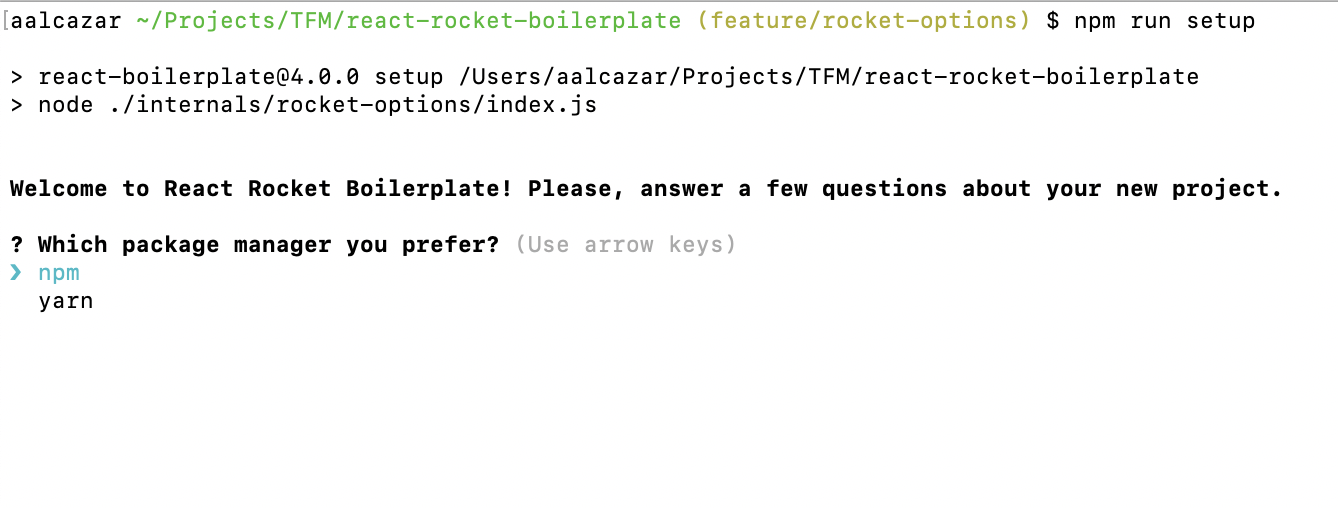
\includegraphics[width=\textwidth]{rocket-generator-1.png}
  \caption{React Rocket Generator - Asking about Package Manager}
  \label{fig:rocket-generator-1}
\end{figure}

\begin{figure}
  \centering
  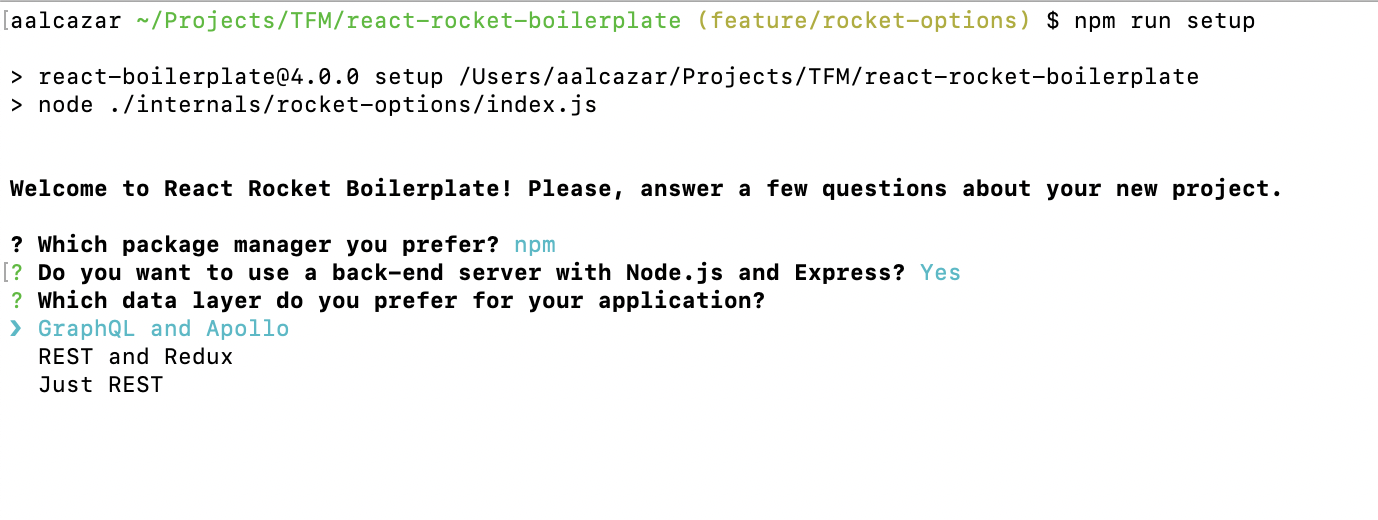
\includegraphics[width=\textwidth]{rocket-generator-2.png}
  \caption{React Rocket Generator - Asking about the API}
  \label{fig:rocket-generator-2}
\end{figure}

\begin{figure}
  \centering
  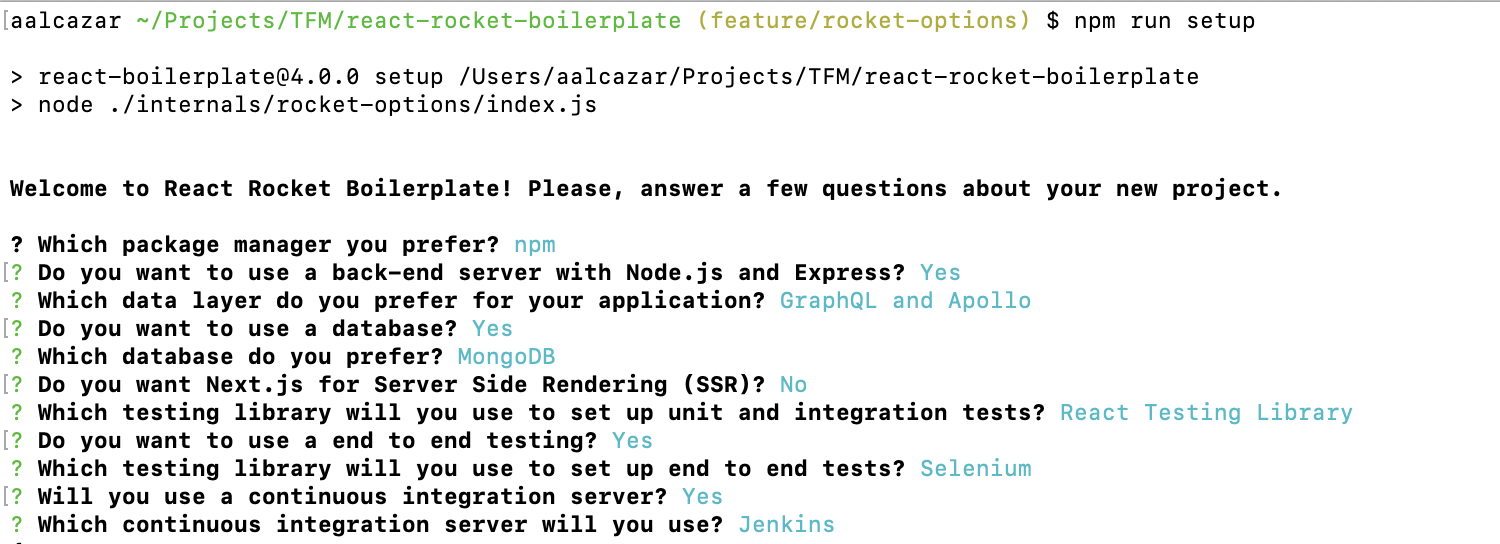
\includegraphics[width=\textwidth]{rocket-generator-3.png}
  \caption{React Rocket Generator - All questions together}
  \label{fig:rocket-generator-3}
\end{figure}

Cabe destacar que el proyecto se ha planteado como un proyecto abierto y la intención es ir incrementando el número de opciones de las que dispone el usuario para que el marco vaya siendo cada vez lo más completo posible. Cómo se puede ampliar el proyecto y cómo se ha planteado la ampliabilidad del proyecto se detalla más adelante en el apartado \nameref{chap:further-steps}.

El marco cuenta con un proyecto modelo para todas las opciones que introduzca el usuario. El proyecto modelo es una simple lista de tareas (ver lista de tareas vacía en la figura \cref{fig:todo-list-1}), en la cual el usuario puede añadir nuevas tareas (\cref{fig:todo-list-2}), marcar y desmarcar las tareas como hechas (\cref{fig:todo-list-3}), modificarlas y borrarlas. Este proyecto modelo ha sido realizado para todas las opciones de las que dispone el marco de trabajo: todos los tipos de base de datos incluídos en \nameref{section:database-manager} y todas las capas de datos incluídas en \nameref{section:data-layer}. Además, se ha cubierto el proyecto modelo con un 98\% de cobertura en pruebas para todos los tipos de proyecto modelo. Las pruebas se han realizado únicamente mediante Jest y React Testing Library (tal y como se comenta en \nameref{section:unit-testing}), pero entra dentro del ámbito del proyecto (tal y como se comenta más adelante en \nameref{chap:further-steps}) dar también soporte a Enzyme. Esto implicará repetir todas las baterías de pruebas para Enzyme.

\begin{figure}
  \centering
  
\includegraphics[width=\textwidth]{todo-list-1.png}
  \caption{React Rocket Todo List - Empty List}
  \label{fig:todo-list-1}
\end{figure}

\begin{figure}
  \centering
  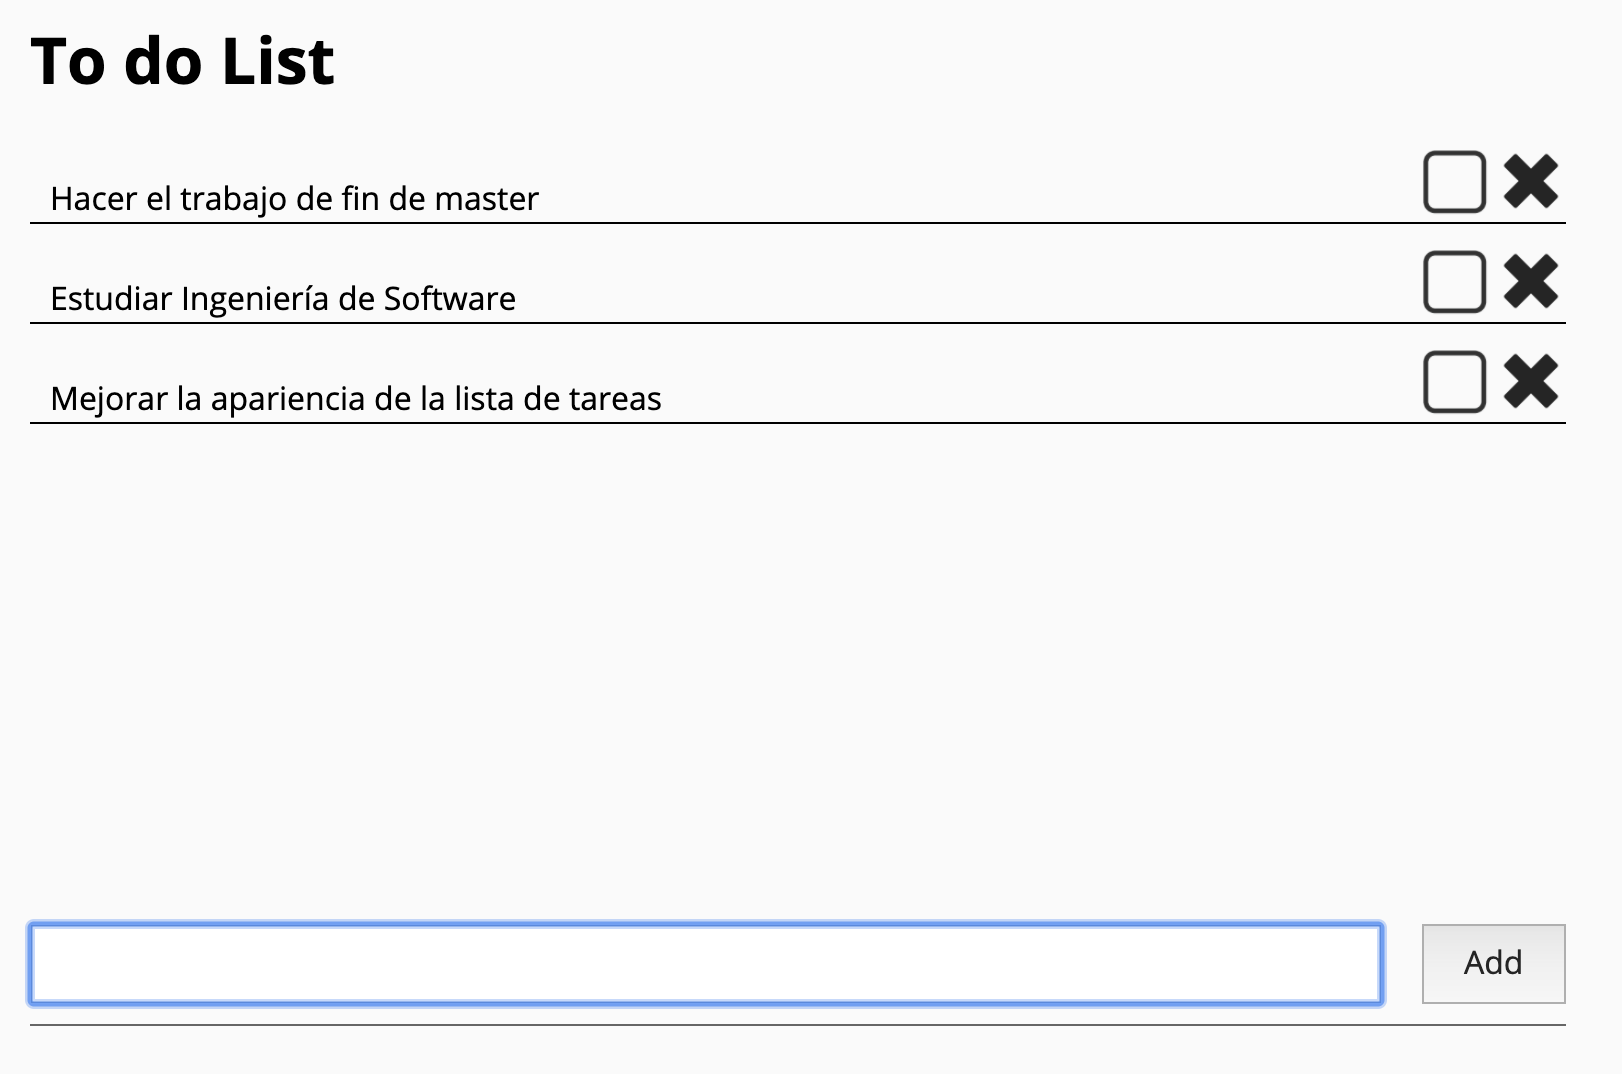
\includegraphics[width=\textwidth]{todo-list-2.png}
  \caption{React Rocket Todo List - Generated 3 items}
  \label{fig:todo-list-2}
\end{figure}

\begin{figure}
  \centering
  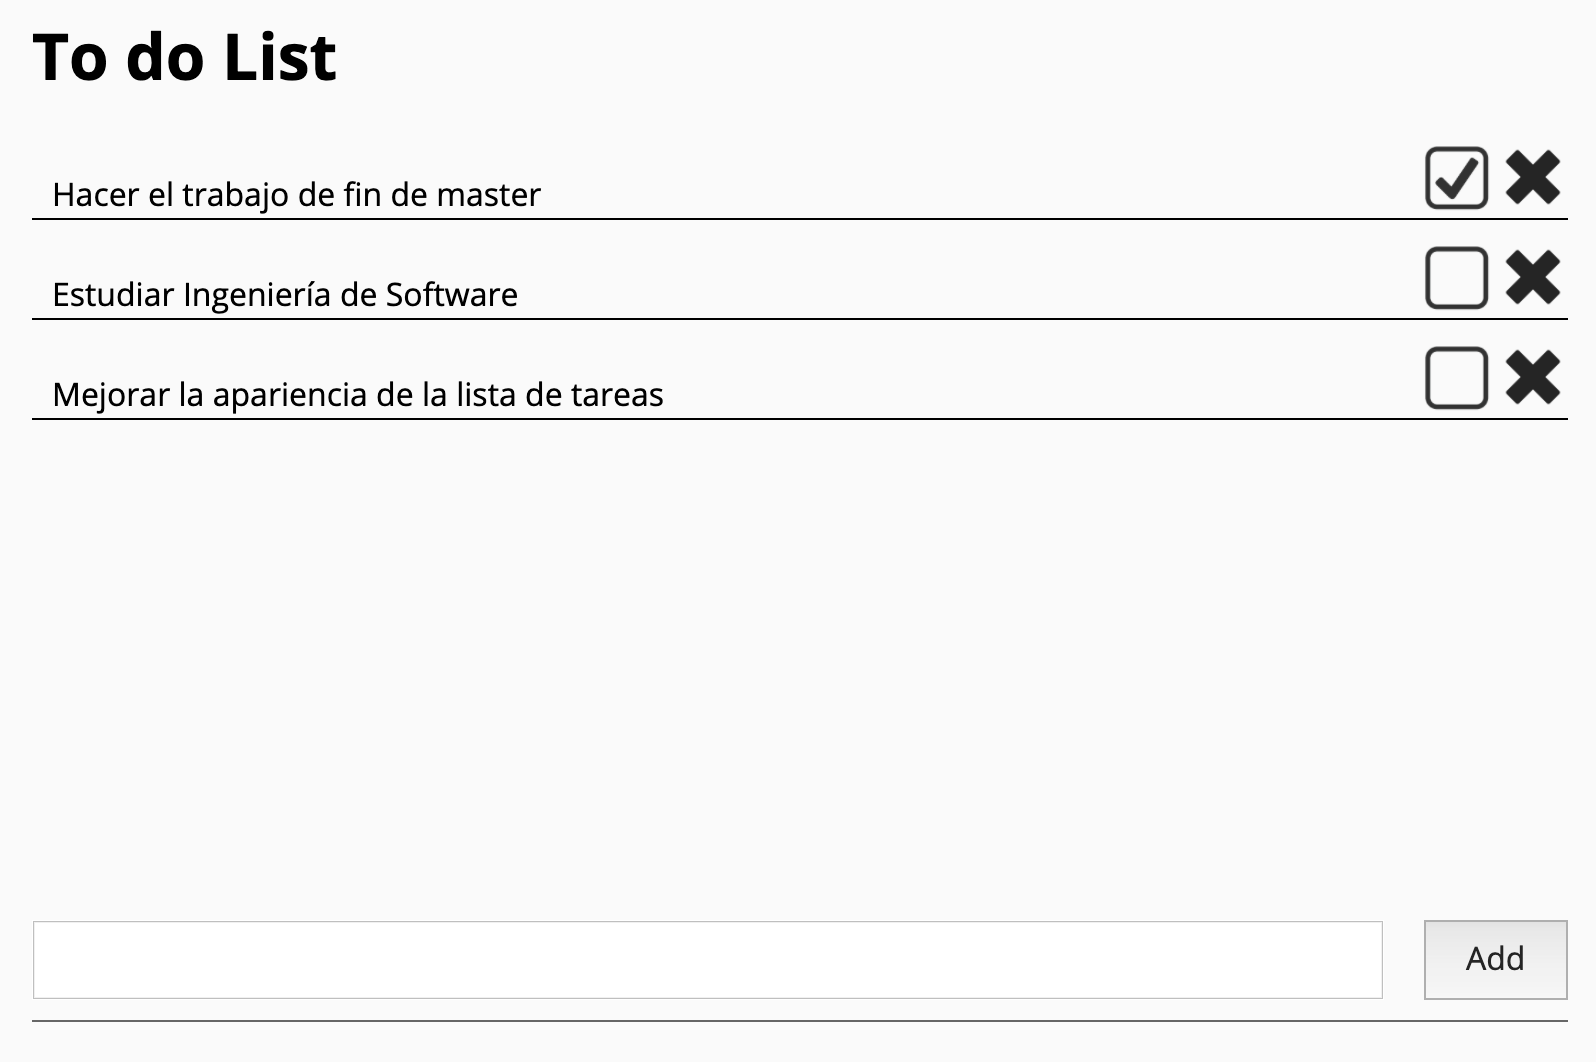
\includegraphics[width=\textwidth]{todo-list-3.png}
  \caption{React Rocket Todo List - Item marked as done}
  \label{fig:todo-list-3}
\end{figure}

Por último, el proyecto cuenta con integración continua integrada. Sin embargo, como esto depende de interacción explícita entre una cuenta registrada en un servidor de git (como Github) y una herramienta de desarrollo continuo (como Jenkins), ha sido imposible automatizar la instalación de la integración continua. Sin embargo, una vez están conectadas ambas herramientas mediante una cuenta con permisos suficientes, se ha logrado automatizar la tarea de integración continua mediante ficheros de configuración (tanto para Jenkins como para CircleCI), tal y como se especifica en el apartado \nameref{chap:ci-cd-detail}.

Con todo esto, el usuario del marco debería tener que hacer los siguientes pasos para poner en mancha un proyecto con este marco:
\begin{enumerate}
\item Clonar el repositorio del proyecto.
\item Ejecutar npm setup.
\item Responder a las preguntas sobre su proyecto. Una vez las termine, el proyecto podrá ser utilizado de forma local con la aplicación modelo descrita anteriormente.
\item Continuar con las instrucciones del README para poner en marcha la integración continua del proyecto.
\end{enumerate}

Como se puede observar, el proyecto es usable con muy poco esfuerzo. La parte más costosa es la de poner en marcha la integración contínua, que es definitivamente algo opcional. Aunque, por otro lado, utilizar este marco carece de sentido si no se pretende realizar un proyecto de calidad con pruebas automáticas e integración contínua.

A lo largo de este capítulo se irá mostrando el detalle completo de todas las partes involucradas en el marco.
